\documentclass{ximera}%handout option removes answers

\usepackage{animate}
\usepackage{tikz}
\usepackage{pgfplots}
\usepackage{pst-3dplot}
\usepackage{pst-solides3d}
\usepackage{pst-math}
\usetikzlibrary{fpu,shadows.blur,shapes.symbols,patterns}
\usetikzlibrary{topaths,intersections,calc,shapes.geometric,arrows,through, positioning}
\usepackage{fp}

\title{Coupled Harmonic Oscillators}
\author{Timothy All}

\begin{abstract}
  We show how to model and solve the system of ODEs that models the coupled, undamped, spring-mass system.
\end{abstract}

\begin{document}
\maketitle


Consider the coupled system pictured below.

\begin{image}
%\begin{animateinline}[controls]{18}
%\multiframe{11}{rTick=0+.1}{
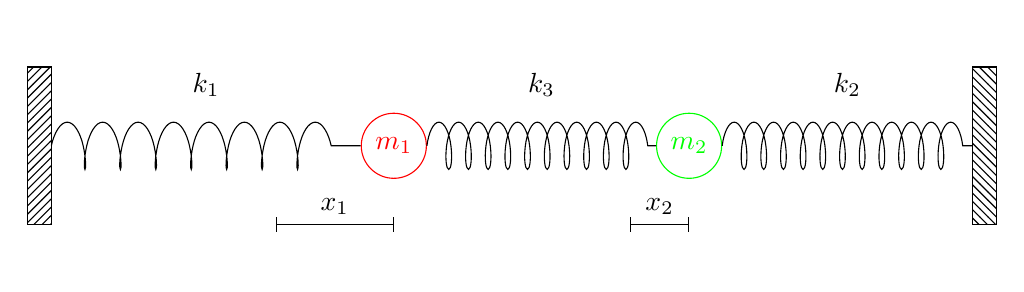
\begin{tikzpicture}[x=1.5cm]
\useasboundingbox (-.1,-1.5) rectangle (8.1,1.5);
\pgfmathsetmacro\rTick{1}
\pgfmathsetmacro\a{2+\rTick}
\pgfmathsetmacro\b{5+\rTick/2}
\pgfmathsetmacro\oa{\a*3/2}
\pgfmathsetmacro\ab{(\b-\a)}
\pgfmathsetmacro\bo{8-\b}

\node[circle,draw,red] (A) at (\a,0) {$m_1$};%2
\node[circle,draw,green] (B) at (\b,0) {$m_2$};%5
%\draw [fill=red] (A) circle (1.5pt);%
%\draw [fill=red] (B) circle (1.5pt);%

\draw [decoration={aspect=0.3, segment length=\oa mm, amplitude=3mm,coil},decorate] (.1,0)--(A) node[midway,above=.5] {$k_1$};%
\draw [decoration={aspect=0.3, segment length=\ab mm, amplitude=3mm,coil},decorate] (A)--(B) node[midway,above=.5] {$k_3$};%
\draw [decoration={aspect=0.3, segment length=\bo mm, amplitude=3mm,coil},decorate] (B)--(7.9,0) node[midway,above=.5] {$k_2$};%

\draw [pattern=north east lines] (-.1,-1) rectangle (.1,1);%

\draw [pattern=north west lines] (7.9,-1) rectangle (8.1,1);

\draw [|-|] (2,0)++(-90:1) --+ (0:\rTick) node[midway,above] {$x_1$};
\draw [|-|] (5,0)++(-90:1) --+ (0:\rTick/2) node[midway,above] {$x_2$};

\end{tikzpicture}
%}
%\end{animateinline}

\end{image}

{\bf Newton's Second Law} says that the sum total force $F$ acting on an object of mass $m$ satisfies $F= \answer{m \cdot a}$, where $a$ is the acceleration. On the other hand, we have {\bf Hooke's Law}: the force $F$ required to stretch a spring $x$ units beyond its natural length is $\answer{k \cdot x}$ where $k$ is some constant depending on the spring. The individual spring constants are in our coupled system are labeled in the image above.

\begin{problem}
The sum total force acting on $m_1$ is $F_1 = \answer{-k_1 x_1 - k_3(x_2-x_1)}$
\end{problem}

\begin{problem}
The sum total force acting on $m_2$ is $F_2 = \answer{-k_2 x_2 + k_3(x_2-x_1)}$
\end{problem}

\begin{problem} The function $x_1(t)$ satisfies the following differential equation:
\[ \answer{m_1 x_1'' = -(k_1-k_3)x_1 -k_3 x_2}\]
\begin{hint} Remember that acceleration is the second derivative of position \end{hint}

\end{problem}

\begin{problem} The function $x_2(t)$ satisfies the following differential equation:
\[ \answer{ m_2 x_2'' = -k_3 x_1 + (k_3-k_2)x_2.}\]
\end{problem}

\[ \graph{sin(ax),a=1} \]

\animategraphics[autoplay,loop]{1}{standalone}{}{}







\end{document}
